% TeX file "introduction"

% Research Module in Econometrics & Statistics 
% Prof. Dr. Liebl & Dr. Christopher Walsh
% Winter 2021/22, M.Sc. Economics, Bonn University
% Xingyu Tao, Xuan Li, Sven Jacobs


\section{Introduction}

In regression analysis, it is often too restrictive to assume a specific structure of the regression function.
Nonparametric methods instead only need minimal smoothness and aim to \enquote{let the data speak for themselves}.
One popular class in nonparametric regression is formed by kernel estimators.
They are known to be simple to understand, to analyze mathematically and to implement on a computer \parencite{Ruppert_1994}.
However, kernel estimators generally suffer from poor behavior near boundaries when the function to be estimated has compact support.
In the literature, this is referred to as boundary effects.

For the theoretical analysis we assume to observe i.i.d.\ data $\{(X_i, Y_i)\}_{i = 1, \dots, n}$
where the random variables $X_1, \dots, X_n$ have density $f$, the so-called design density.
Importantly, we assume that $X_i \in [a, b] \subset \mathbb{R}$.
The problem is now to estimate the unknown function $m$ from the sample of noisy data:
\begin{equation}
	Y_i = m(X_i) + \epsilon_i \,.
\end{equation}
For the error term $\epsilon_i$ we state that $\E[\epsilon_i \,|\, X = X_i] = 0$ and $\Var(\epsilon_i \,|\, X = X_i) = \sigma^2(X_i)$.
In the considered random design the target $m$ is then the conditional expectation function, i.e.\ $m(X_i) = \E[Y_i \,|\, X = X_i]$.

If the function $m$ is believed to be smooth, we should obtain a reasonable estimate at a point $x$ by taking a local average of observations close to $x$.
Following this line, a kernel estimator approximates $m(x)$ by a weighted local average of the $Y_i$'s, where the weights are given by a kernel.
The standard kernel estimator, the Nadaraya-Watson estimator, is defined as
\begin{equation} \label{eq:nw}
	\hat{m}_{\NW}(x) = \sum_{i = 1}^{n} w(x, X_i, h) Y_i =
	\sum_{i = 1}^{n} \frac{K \left( \frac{X_i - x}{h} \right)}{\sum_{j = 1}^{n} K \left( \frac{X_j - x}{h} \right)} Y_i \,, 
\end{equation}
with kernel function $K$ and bandwidth $h$.
The weight function $K$ is usually chosen to be a unimodal probability density function which is symmetric about zero.
A collection of prominent choices is presented in Appendix~\hyperref[appendix_2]{2}.
The bandwidth $h$ is a smoothing parameter controlling how fast the weights decrease in $|X_i - x|$.
As we see later, the kernel choice is less important, whereas the bandwidth has a crucial impact on the estimation.
Figure~\ref{fig:nw_interior} shows how the Nadaraya-Watson estimator typically forms an estimate.
The estimate at $x = 0.5$ is computed as a locally weighted average of those observations falling into the yellow-shaded window, whose size is determined by the bandwidth $h = 0.2$. 
The assigned weights are proportional to the plotted Epanechnikov kernel (see Table~\ref{tab:kernels}).
The resulting estimate is nearly unbiased.

In Figure~\ref{fig:nw} we notice, however, that near the boundaries zero and one the Nadaraya-Watson estimate differs substantially from the true curve.
Figure~\ref{fig:nw_boundary} reveals why the estimate at the lower boundary $x = 0$ is upwards biased.
Since we only observe data of the regressor greater than zero, the left half of the kernel window is devoid of data.
The local averaging process gets asymmetric and the positive slope of the regression function in the interval $[0, 0.2]$ induces marked bias.
These boundary effects are visually disturbing in practice (also consider Figure~\ref{fig:boundary_effects_linear}),
but additionally the bias results in a slower rate of convergence near the boundary compared to points in the interior.
Both together indicates the need for boundary modifications.

\begin{figure}
	\centering
	\begin{subfigure}{0.75\textwidth}
		\centering
		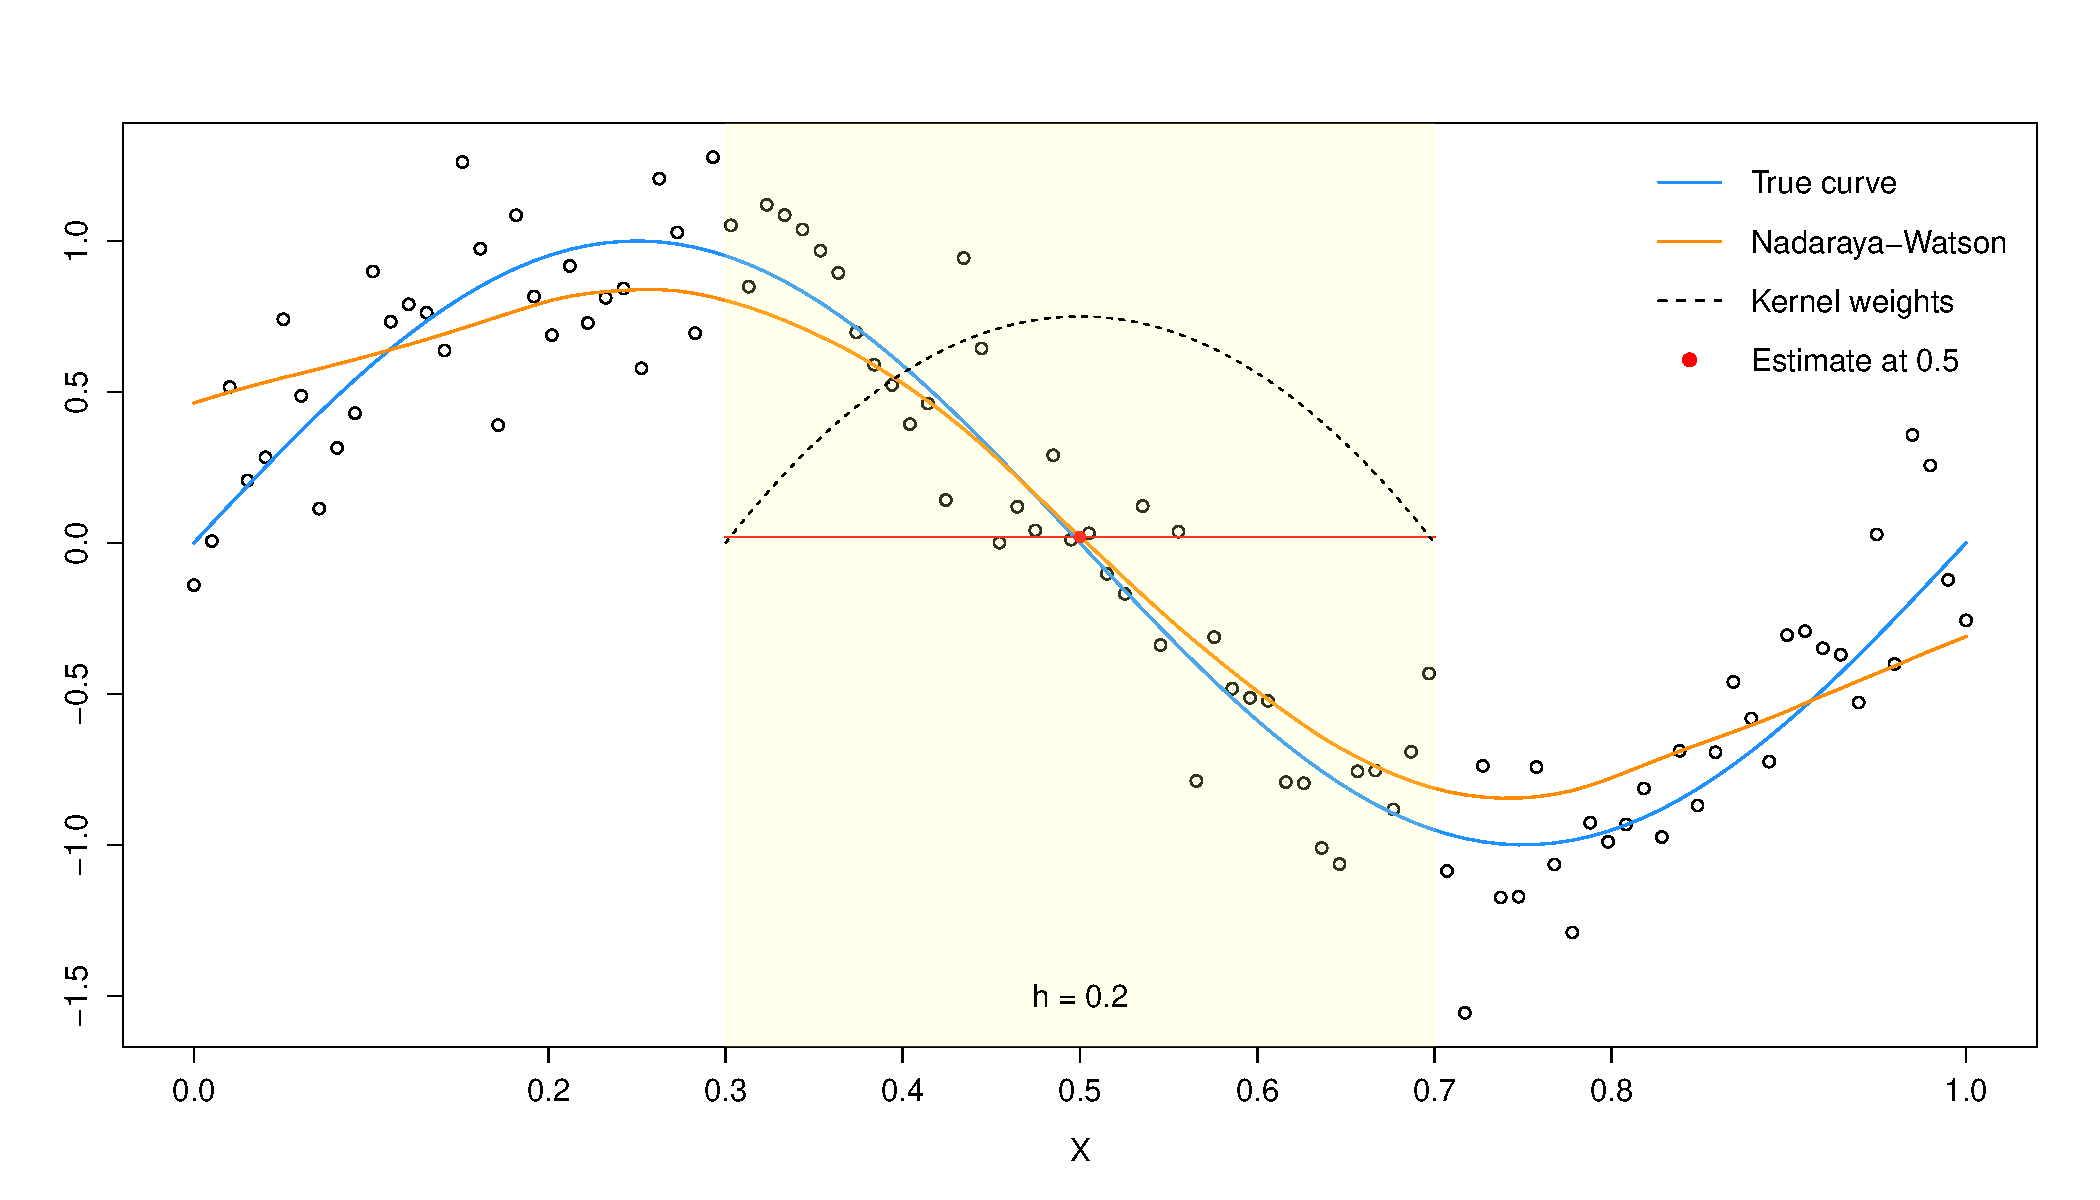
\includegraphics[trim=20 15 20 50, clip, width=\textwidth]{figure_01a.pdf}
		\caption{Estimation in the interior}
		\label{fig:nw_interior}
	\end{subfigure}

	\begin{subfigure}{0.75\textwidth}
		\centering
		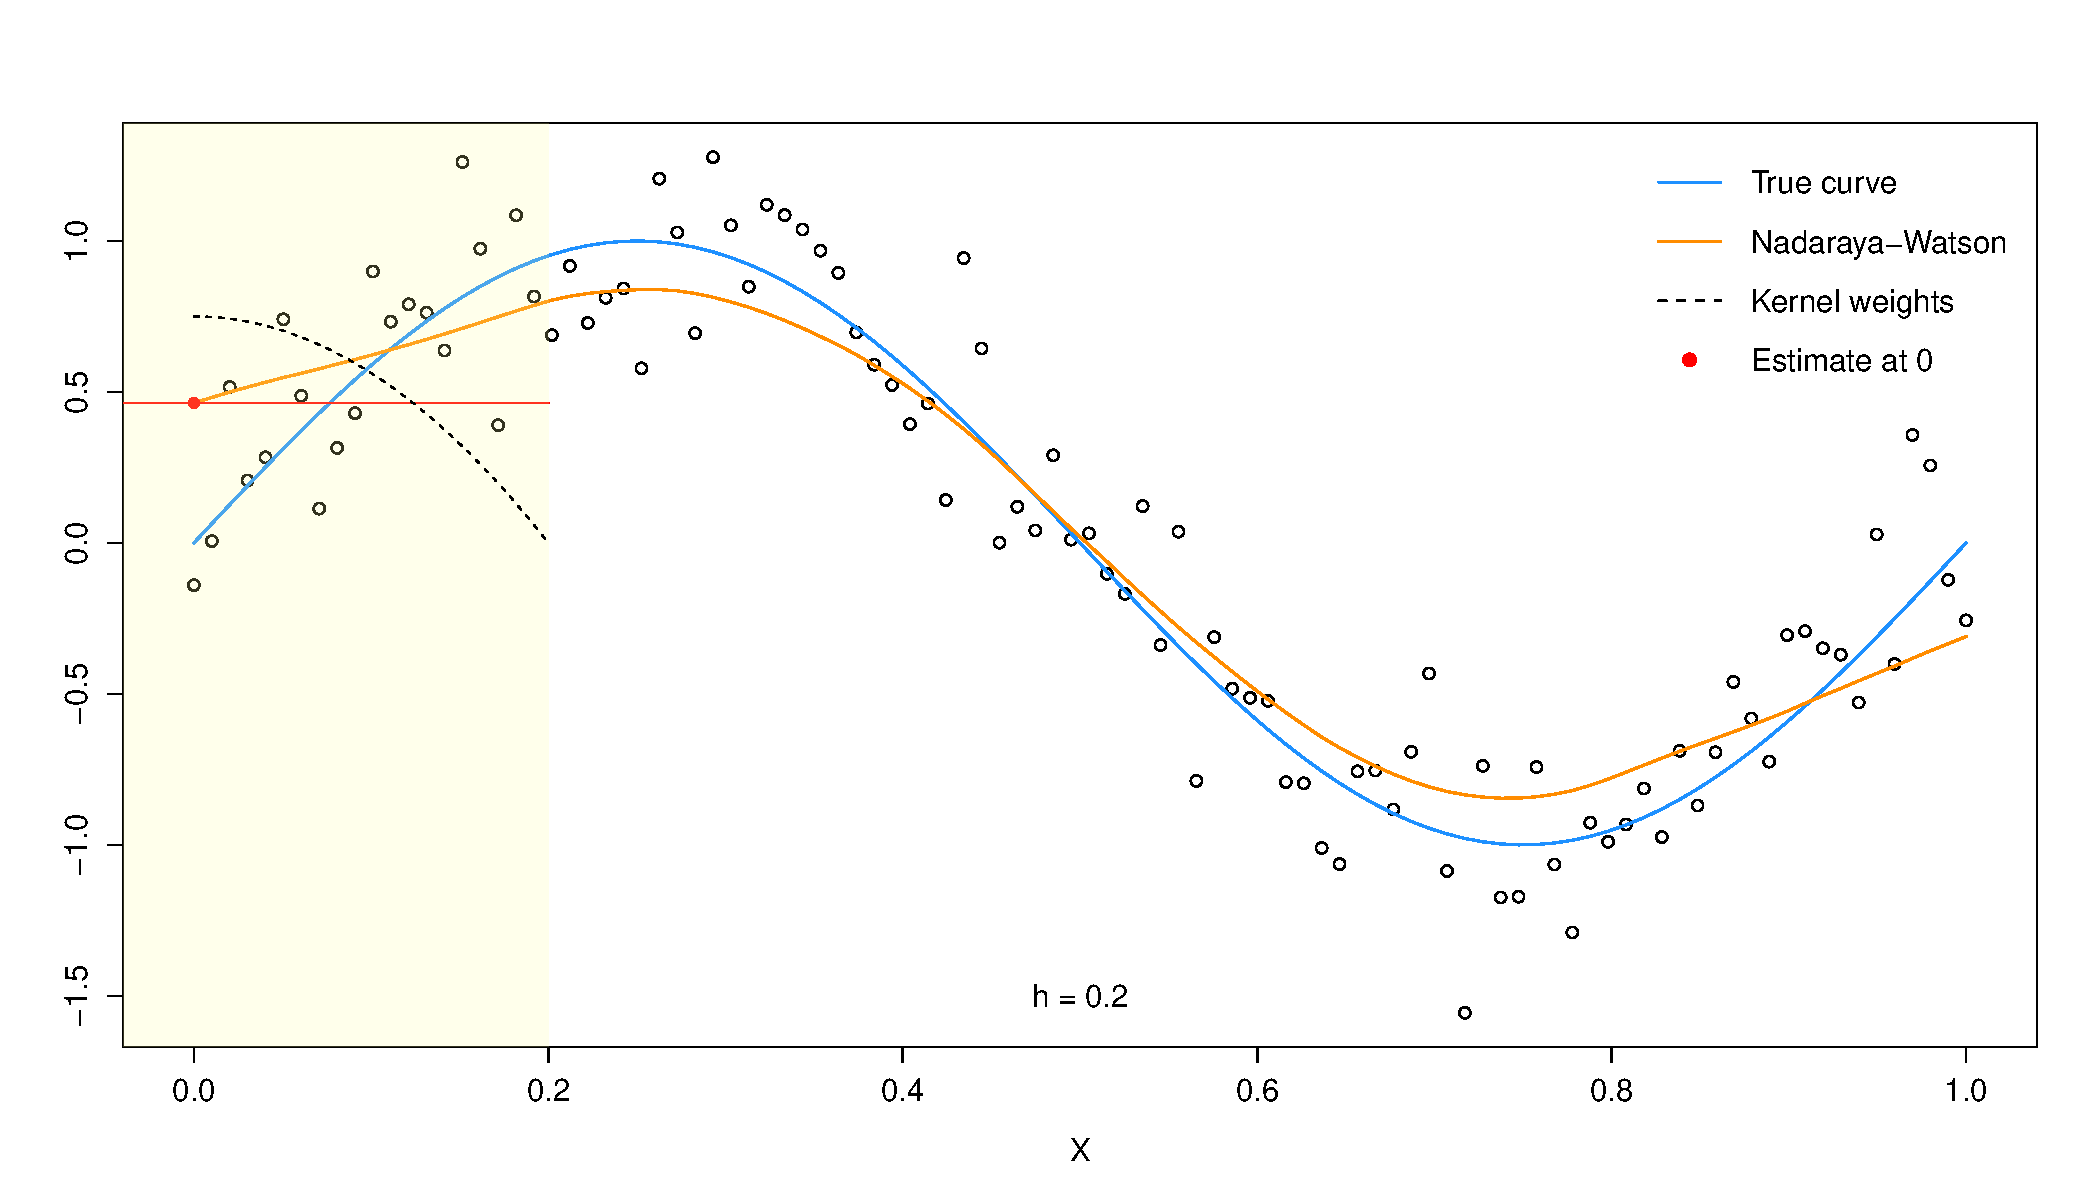
\includegraphics[trim=20 15 20 50, clip, width=\textwidth]{figure_01b.pdf}
		\caption{Estimation at the boundary}
		\label{fig:nw_boundary}
	\end{subfigure}
	\caption{Illustration of the estimation procedure underlying the Nadaraya-Watson estimator for 100 simulated observations (empty circles)}
	\label{fig:nw}
\end{figure}

Several methods have been proposed to overcome the boundary problem.
We focus on the two most relevant approaches.
First, the adjustment of the Nadaraya-Watson estimator by using special boundary kernels to asymptotically correct for the bias.
Second, local linear regression which locally fits a weighted regression line and is known to automatically correct the bias exactly to first order \parencite{Hastie_1993}.
The goal of this paper is then twofold.
Describing theoretically how both methods improve on the standard Nadaraya-Watson estimator.
And investigating the finite sample properties by means of Monte-Carlo simulations and a real-data application.

The Nadaraya-Watson estimator was independently proposed by \textcite{Nadaraya_1964} and \textcite{Watson_1964}.
The idea of locally weighted regression appeared first in \textcite{Stone_1977} and \textcite{Cleveland_1979}.
However, the favorable properties of the local linear estimator including boundary adaption were shown by
\textcite{Fan_1992} and \textcite{Fan_Gijbels_1992}.
\textcite{Ruppert_1994} extended the findings to the multidimensional setting.
\textcite{Gasser_1979} suggested the use of boundary kernels, but only provided ad hoc solutions.
Explicit formulas for polynomial boundary kernels are derived in \citeauthor{Müller_1991} (\citeyear{Müller_1991}, \citeyear{Müller_1993}) and \textcite{Müller_1994}.
\textcite{Gasser_1985} and \textcite{Granovsky_1991} also discuss boundary kernels.
Other methods to reduce the boundary bias include a generalized jackknife combination of two kernel estimators with different bandwidths
\parencite{Rice_1984, Kyung-Joon_1998}, as well as data reflection \parencite{Hall_1991}.

The remainder of the paper is structured as follows.
In the next section we formally introduce local linear regression and compare it to the Nadaraya-Watson estimator,
both theoretically and graphically.
Section~\ref{sec:boundary_kernels} discusses the idea and functioning of boundary kernels.
In Section~\ref{sec:simulation} we present a Monte-Carlo simulation study to compare the finite sample behavior of the methods.
An important application is given in Section~\ref{sec:application}:
the nonparametric estimation of causal effects in the regression discontinuity design (RDD).
Section~\ref{sec:conclusion} concludes.
The appendix contains proofs, information about kernels and additional figures and tables.